\section{Learning Objectives}\label{learning-objectives}

\begin{enumerate}
\def\labelenumi{\arabic{enumi})}
\item
  Discuss the process of identifying a relevant project, and appraise
  his or her own performance
\item
  Justify the choice of project made. Identify relationship of personal
  interest and learning that has taken part in other parts of the
  course.
\item
  Identify the methodological, organisational and technological
  challenges to the successful planning and carrying out of the project.
  Justify approaches taken on these issues.
\item
  Demonstrate a clear grasp of the subject matter and a full
  understanding of principles.
\item
  Develop and work to a specification and set requirements.
\item
  Demonstrate independent work.
\item
  Coordinate all activities needed to produce the agreed deliverables.
\item
  Show competence to document appropriately and demonstrate the results
  of their work.
\item
  Demonstrate an awareness of the relevant professional, social, legal
  and ethical aspects.
\item
  Critically appraise his or her own performance in undertaking the
  project itself and identify the lessons learned from undertaking it.
\end{enumerate}

\section{Project Timetable}\label{project-timetable}

\begin{figure}[htbp]
\centering
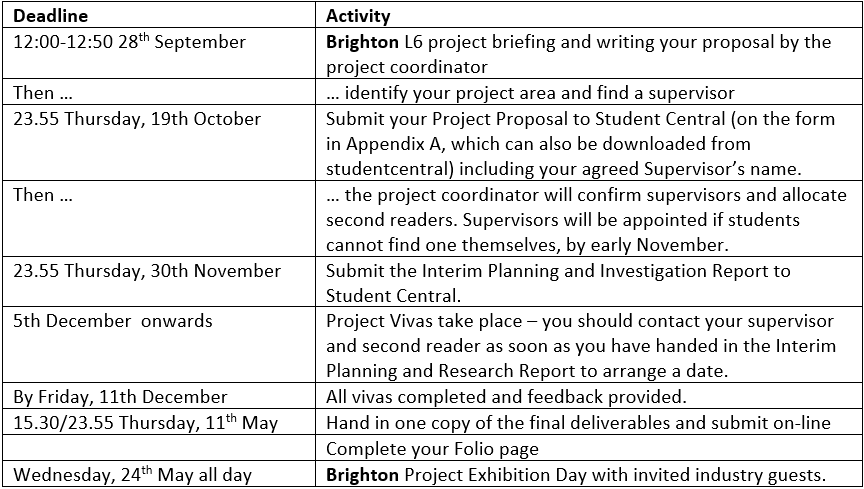
\includegraphics{./Images/projecttimetable.png}
\caption{Project timetable}
\end{figure}

\section{How to show planning}\label{how-to-show-planning}

\begin{itemize}
\item
  Outline goals and targets for project. Small goals that are achievable
  over a short time span that build to a larger goal.
\item
  Outline a weekly/monthly plan on achieving my end results
\item
  Research and gain background information in the targeted field.
\end{itemize}

\section{How to show work ethic}\label{how-to-show-work-ethic}

\begin{itemize}
\tightlist
\item
  Keep a work log.
\item
  Using version control (GitHub) to show work and progress.
\item
  End report.
\end{itemize}

\section{Showing results}\label{showing-results}

\begin{itemize}
\tightlist
\item
  End report. (90\%)
\item
  Show the project in full
\item
  Viva/oral exam and presentation to outline what I have done. (10\%)
\end{itemize}

\section{Breakdown of learning}\label{breakdown-of-learning}

Total hours of learning 400

\begin{itemize}
\tightlist
\item
  10h Taught
\item
  12h Supervised
\item
  378h Independent
\end{itemize}

Assuming 30 weeks (During term times) = approx 13 hours per week / 2
hours per day.

Tuesday is a free day so 6 hours will be used as follows:

\begin{itemize}
\tightlist
\item
  10:00 - 12:00 = Working on project. (2h)
\item
  12:00 - 13:00 = Lunch break
\item
  13:00 - 15:00 = Working on project. (2h)
\item
  15:00 - 15:30 = Short break.
\item
  15:30 - 17:30 = Working on project. (2h)
\end{itemize}

For the last work session most work will be updating documentation and
pushing any completions to version control.

\section{Mark scheme}\label{mark-scheme}

\begin{figure}[htbp]
\centering
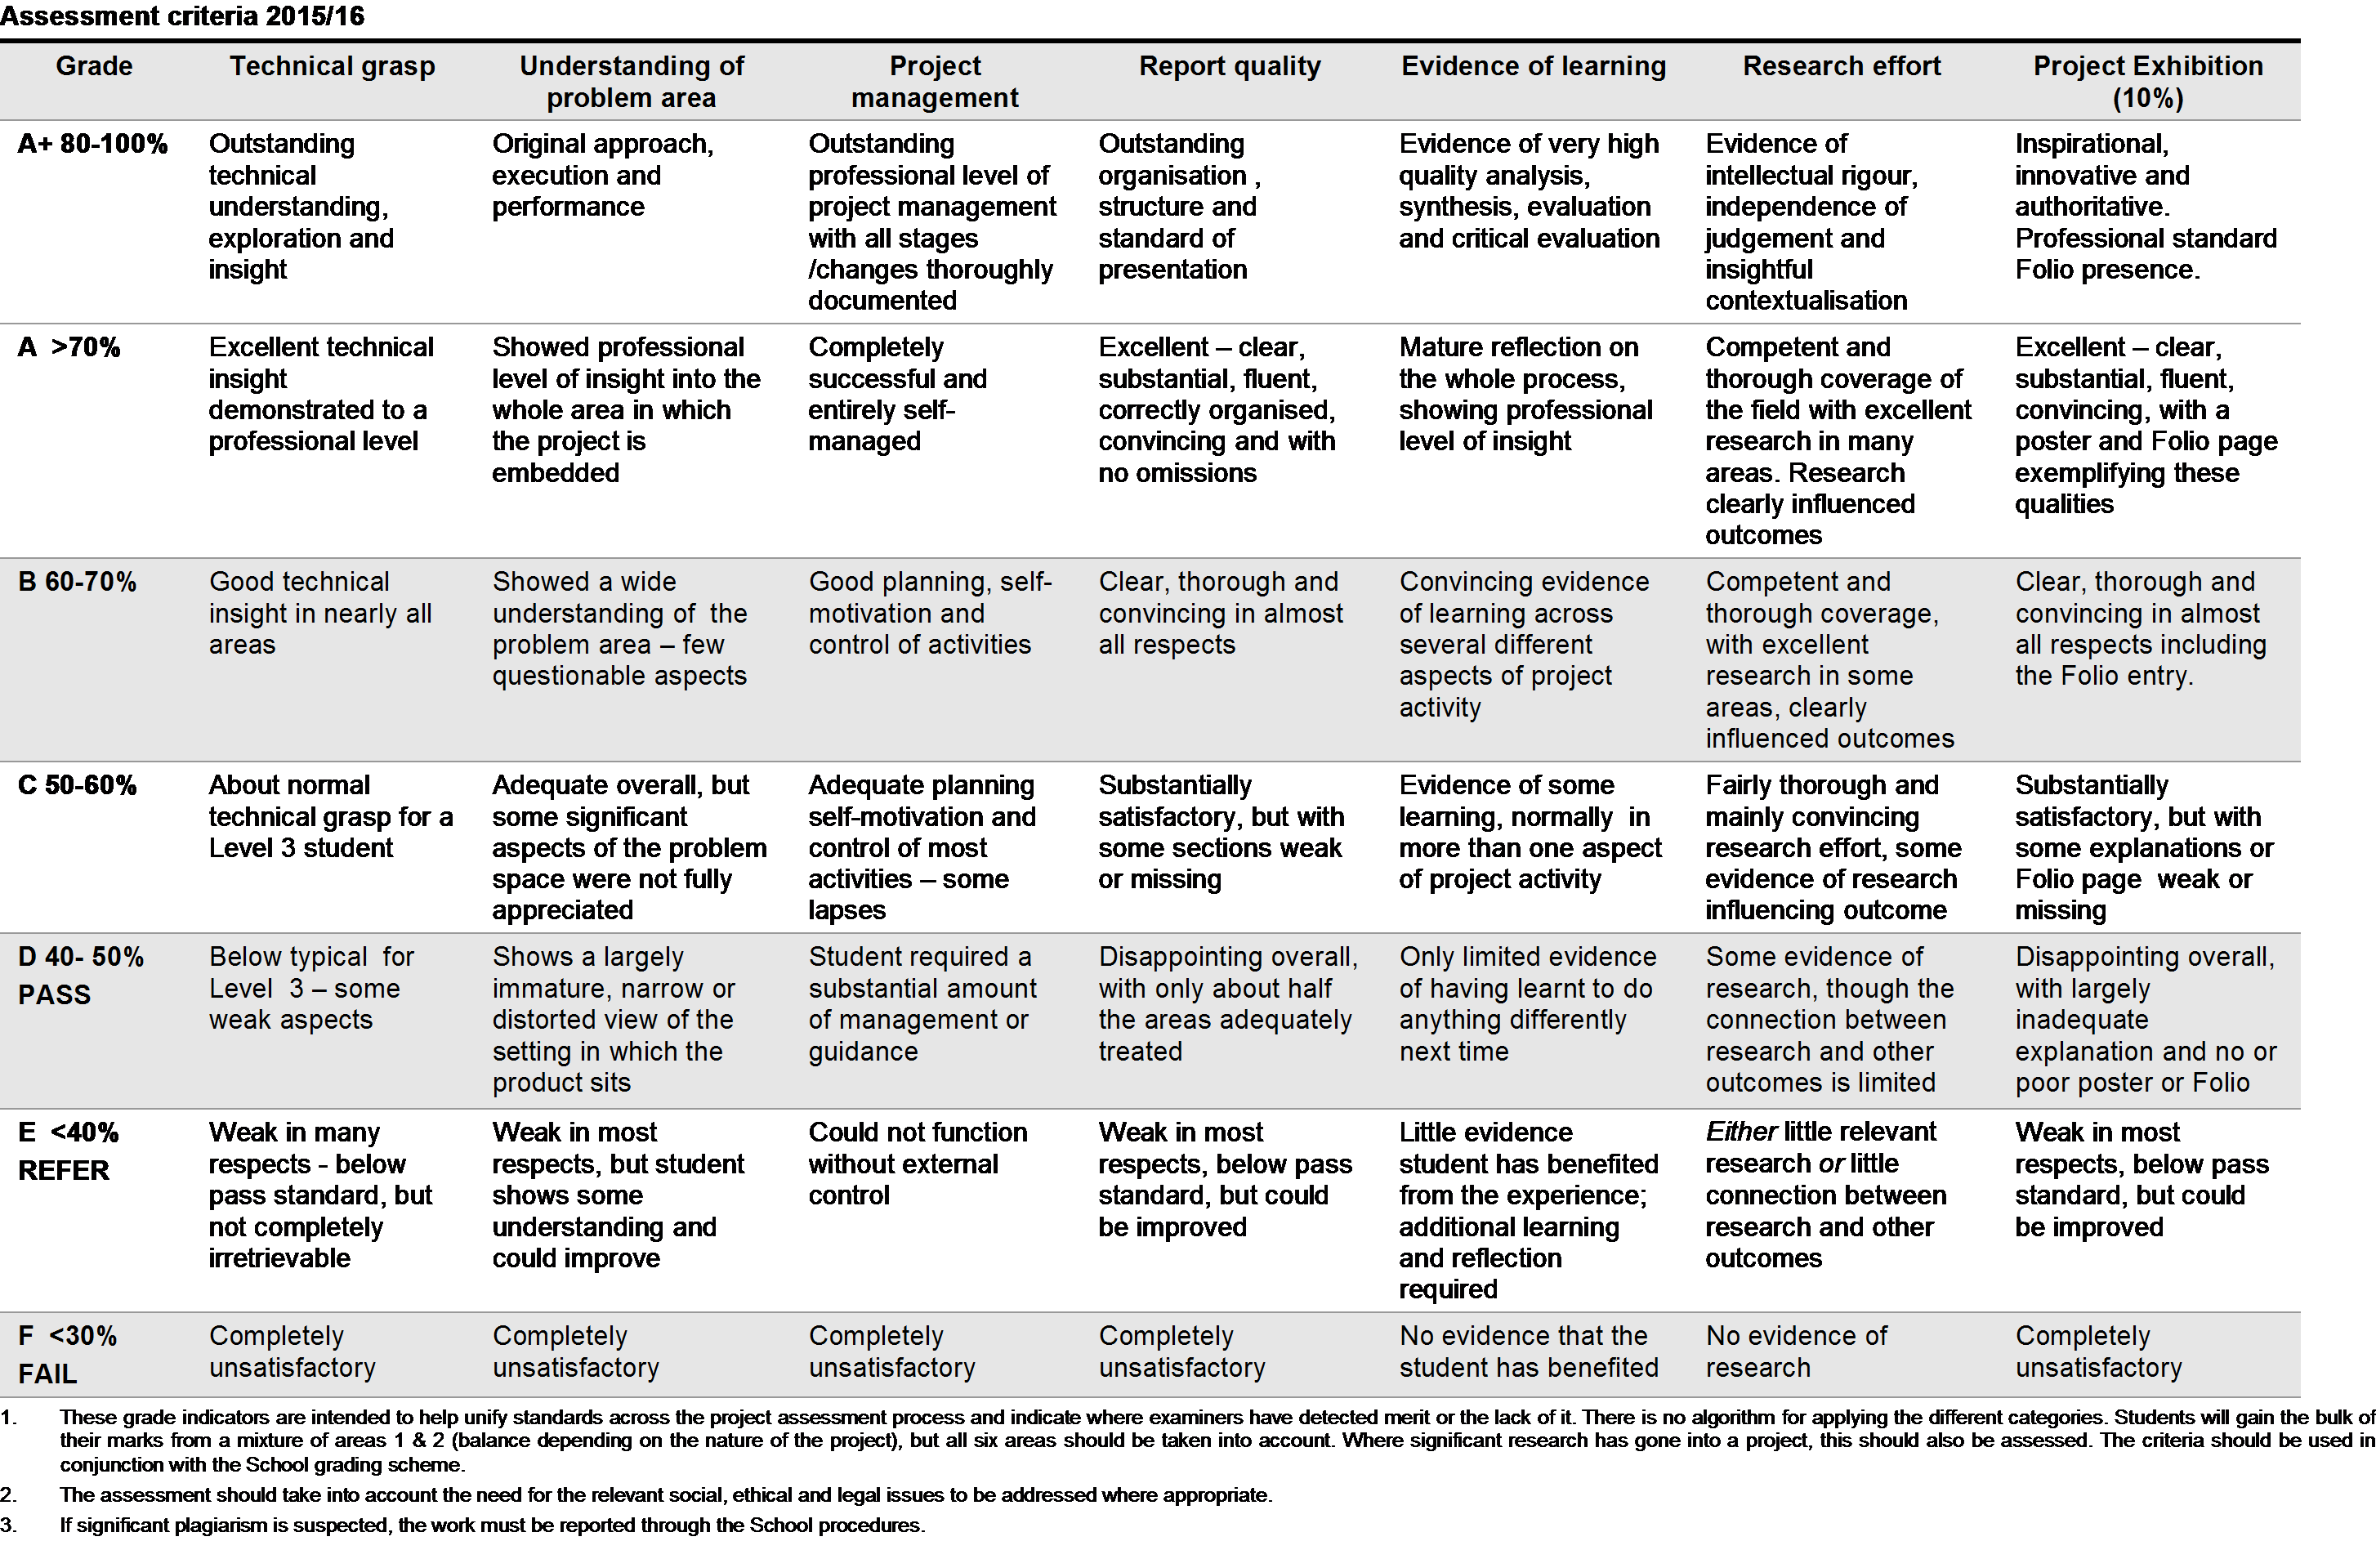
\includegraphics{./Images/markscheme.png}
\caption{Mark Scheme}
\end{figure}

\section{Project proposal}\label{project-proposal}

Find in
\href{https://studentcentral.brighton.ac.uk/bbcswebdav/pid-2748868-dt-content-rid-5130686_1/xid-5130686_1}{project
handbook}
